%% ------------------------------------------------------------------------- %%
\chapter{Abordagem}
\label{cap:abordagem}


Conforme citado no capítulo~\ref{cap:trabalhos-relacionados}, uma técnica muito utilizada para o problema de \textit{code retrieval} é o \textit{joint embedding}. Para utilizar esta técnica de \textit{joint embedding}, três fatores devem ser levados em consideração:

\begin{itemize}
    \item Representação de cada palavra de uma sentença ou trecho de código-fonte
    \item Representação da sentença e do trecho de código-fonte
    \item Função objetivo do modelo
\end{itemize}

\section{Representação de cada palavra de uma sentença ou trecho de código-fonte}
\label{sec:abordagem-representacao-token}

As questões e os trechos de código-fonte são compostas por palavras, pontuações, separadores e caracteres de símbolos e operadores matemáticos. Para as questões, que são descritas em linguagem natural, iremos representá-las como um vetor formado por uma sequência de palavaras removendo os caracteres de acento e pontuação.

No caso do código-fonte, iremos partir da  mesma hipótese que utilizamos em um artigo. Esta hipótese foi levantada por \cite{Allamanis:2018:SML} e diz que software é uma forma de comunicação humana e tem propriedades estatísticas similares a corpora de linguagem natural. A partir disto, iremos aplicar os mesmos procedimentos adotados para as questões aos trechos de código-fonte. Os trechos de código-fonte terão as pontuações e caracteres especiais removidos e serão tratados como uma sequência de palavras.

No nosso caso, tanto as questões e os trechos de código-fonte serão representados por um vetor formado por uma sequência de palavras. E para cada palavra no vetor, devemos definir uma representação.

De acordo com \cite{Goodfellow-et-al-2016:representation-learning}, as redes neurais generalizam bem quando as palavras são representadas através de vetores de representação distribuída. E conforme o próprio \cite{Goodfellow-et-al-2016:representation-learning}, uma boa representação deve auxiliar na aprendizagem de uma tarefa posterior. No nosso caso, as representações devem auxiliar a tarefa de aprender a encontrar uma correlação entre as questões e os trechos de código-fonte mais relevantes.

Neste trabalho, cada palavra será representada através de um vetor de representação distribuída. Para mapear as palavras para vetores de representação distribuída, utilizaremos inicialmente o algoritmo não-supervisionado \textit{word2vec}. Utilizaremos o \textit{word2vec} com \textit{skip-gram}. O \textit{skip-gram} prediz as palavras do contexto a partir de uma palavra alvo. Diferente do CBoW que prediz a palavra alvo a partir das palavras do contexto. A complexidade do algoritmo \textit{skip-gram} é O(n), enquanto CBoW é exponencial \todo{encontrar referencia complexity function}. 

O \textit{word2vec} irá mapear cada palavra para um espaço vetorial $\mathbb{R}^{d}$. Seja $\mathbb{V}_{q}$ o conjunto de palavras das questões, e $\mathbb{V}_{c}$ o conjunto de palavras presentes nos trechos de código-fonte. Para cada palavra $v_{q} \in \mathbb{V}_{q}$ e $v_{c} \in \mathbb{V}_c$, teremos:

\begin{equation}
    f: v_{q} \rightarrow t_{q}, t_{q} \in \mathbb{R}^{d}
\end{equation}

\begin{equation}
    f: v_{c} \rightarrow t_{c}, t_{c} \in \mathbb{R}^{d}
\end{equation}
Onde $f$ é o \textit{word2vec} com o algoritmo \textit{skip-gram}. $f$ irá mapear cada palavra pertencente a um vocabulário a uma matriz $\bm{T}$.
No nosso caso, teremos duas matrizes: $\bm{T}_{q}^{|\mathbb{V}_{q}| X d}$ e outra $\bm{T}_{c}^{|\mathbb{V}_{c}| X d}$, onde $|\mathbb{V}_{q}|$ e $|\mathbb{V}_{c}|$ são o tamanho do vocabulário das questões e trechos de código-fonte, respectivamente. E $d$ é a dimensão do vetor de representação distribuída.

\section{Representação da sentença e do trecho de código-fonte}

Com cada palavra representada por um vetor de representação distribuída, o próximo passo é combiná-los para obter uma representação para a questão e o trecho de código-fonte. A partir de agora, cada questão ou trecho de código-fonte será representada por um vetor $\bm{x}$, onde $x = \{ \bm{x}(1), \bm{x}(2), . . ., \bm{x}(n) \}$, tal que $\bm{x}(w) \in \mathbb{R}^{d}$ e $w$ é uma palavra presente no vocabulário da questão ou trecho de código-fonte. 

Lembrando que neste trabalho, temos duas matrizes de representação distribuída, $\bm{T}_{q}$ e $\bm{T}_{c}$. Para fins de simplificação, quando utilizarmos $\bm{x}$, $\bm{x}$ pode ser $\bm{x} = \{ t_{q}(1), t_{q}(2), . . ., t_{q}(n)\}$, $t_{q}(i) \in \bm{T}_{q}, 1 \leq i \leq n$ ou pode ser $\bm{x} = \{ t_{c}(1), t_{c}(2), . . ., t_{c}(n)\}$, $t_{c}(i) \in \bm{T}_{c}, 1 \leq i \leq n$.


Iremos avaliar duas formas de representar as questões e trechos de código-fonte. Uma abordagem é utilizando uma rede neural recorrente bi-LSTM com uma camada CNN posterior. E a outra abordagem é uma rede CNN apenas.

\subsection{Representação através de bi-LSTM com CNN}

Utilizando o LSTM, a partir de um vetor $\bm{x} = \{ \bm{x}(1), \bm{x}(2), . . ., \bm{x}(n) \}$, onde $\bm{x}(t)$ é um vetor de representação de dimensão $d$. O valor do vetor de \textit{hidden} $\bm{h}(t)$ (tamanho $H$) na iteração $t$ é:

\begin{equation}
    i_{t} = \sigma(\bm{W}_{i}\bm{x}(t) + \bm{U}_{i}\bm{h}(t - 1) + \bm{b}_{i})
\end{equation}
\begin{equation}
    f_{t} = \sigma(\bm{W}_{f}\bm{x}(t) + \bm{U}_{f}\bm{h}(t - 1) + \bm{b}_{f})
\end{equation}
\begin{equation}
    o_{t} = \sigma(\bm{W}_{o}\bm{x}(t) + \bm{U}_{o}\bm{h}(t - 1) + \bm{b}_{o})
\end{equation}
\begin{equation}
    \bar{C}_{t} = tanh(\bm{W}_{c}\bm{x}(t) + \bm{U}_{c}\bm{h}(t - 1) + \bm{b}_{c})
\end{equation}
\begin{equation}
    C_{t} = i_{t} * \bar{C}_t + f_{t} * C_{t - 1}
\end{equation}
\begin{equation}
    \bm{h}_{t} = o_{t} * tanh(C_{t})
\end{equation}

No caso do bi-LSTM, teremos duas redes LSTM, uma rede que lê o vetor $\overrightarrow{\bm{x}}$ na ordem da primeira para a última palavra, $\bm{x}(1), \bm{x}(2), . . ., \bm{x}(n)$. E a outra rede LSTM vai ler na ordem inversa, $\overleftarrow{\bm{x}}$, $\bm{x}(n), \bm{x}(n - 1), . . ., \bm{x}(1)$. Teremos dois vetores \textit{hidden}.

\subsection{CNN}

\begin{equation}
    o_{F}(t) = tanh \left[\left(\sum_{i=0}^{m - 1} \bm{h}(t-1)^{T}\bm{F}(i)\right) + b\right]
\end{equation}

$$
\begin{pmatrix} 
a & b \\
c & d 
\end{pmatrix}
\odot
\begin{pmatrix} 
a & b \\
c & d 
\end{pmatrix}
=
\begin{pmatrix} 
a & b \\
c & d 
\end{pmatrix}
$$

Para representar uma questão ou trecho de código-fonte, podemos calcular a média dos vetores de resultado $\bm{h} = \{ \bm{h}_{1}, \bm{h}_{2}, . . ., \bm{h}_t \}$ após $t$ iterações, por exemplo.


No nosso trabalho, utilizaremos o mesmo procedimento para representar as questões e os trechos de código-fonte. Se




Conforme o capítulo~\ref{cap:trabalhos-relacionados}, há várias pesquisas sobre o problema de perguntas e respostas no processamento de linguagem natural. Porém, como observado pelo trabalho da \cite{yao-2018} e apontado na seção~\ref{sec:algumas_referencias}, não há muita pesquisa sobre o problema de pares de perguntas e códigos-fontes. A partir de 2014, o StackOverFlow passou a disponibilizar a base de dados livremente. Diversas pesquisas foram feitas utilizando esta base de dados. E uma frente explorada pela \cite{yao-2018} e outros pesquisadores, é tentar resolver o problema de pergunta e resposta utilizando os dados do \textit{StackOverFlow}.

\subsection{Code Embedding}

Conforme \cite{cambronero-deep-learning-code-search:2019}, a partir dos \textit{token embeddings} podemos gerar uma representação para os trechos de código-fonte.

Os trechos de código-fonte podemm ser tratados como uma \textit{bag} de palavras. Quer dizer, a ordem dos termos não é levada em consideração \citep{cambronero-deep-learning-code-search:2019}.

\todo{adicionar mais informações}

\todo{adicionar definição do toke embedding}

Por exemplo:

\todo{adicionar um exemplo}



Ou a ordem pode ser levada em consideração. E neste caso, pode utilizar uma rede neural recorrente. Por exemplo, uma rede bi-LSTM. 

\todo{adicionar a fóruma do bi-LSTM}

%------------------------------------------------------
\section{Problema de pares de perguntas e códigos-fontes do \textit{StackOverFlow}}

O problema de pares de perguntas e códigos-fontes já foi discutido na seção~\ref{sec:algumas_referencias}. E um dos obstáculos mencionados, é a obtenção de dados para o treinamento de modelos supervisionados. Desde 2014, o site \textit{StackOverFlow} disponibiliza sua base de perguntas e respostas através do site \cite{sof-2019}. Estes dados também podem ser consultados através do site \textit{BigQuery} do \cite{bigquery-2019} também. Numa consulta rápida, até 20 de março de 2019, havia mais de 17 milhões de perguntas em diversos tópicos de programação. Dúvidas sobre Python e SQL totalizam juntas mais de 2 milhões e meio.

\begin{figure}[h]
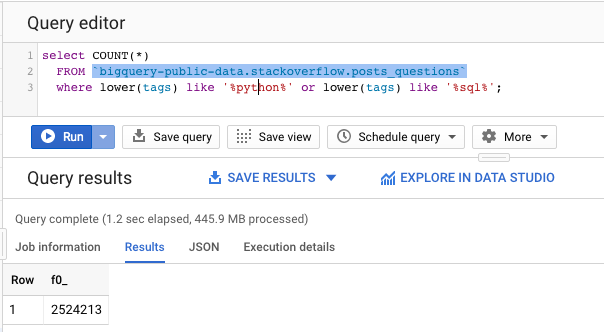
\includegraphics[width=12cm]{figuras/cap-problema/post-questions-python-sql-total.png}
\caption{Total de perguntas sobre Python e SQL no \textit{StackOverFlow} até 20 de março de 2019. Google and the Google logo are registered trademarks of Google LLC, used with permission.}
\label{fig:bigquery-total-questions-python-sql-stackoverflow}
\end{figure}

Somente com estes números, vê-se o potencial do \textit{StackOverFlow} como fonte de perguntas em linguagem natural e a sua solução em código fonte \cite{yao-2018}. Mas antes de utilizá-lo como fonte, é necessário levar em consideração quais assuntos é permitido fazer a pergunta. De acordo com o guia de boas práticas do \cite{stackoverflow-questions-topics-2019}, são permitidas perguntas sobre:

\begin{itemize}
    \item um problema específico de programação
    \item um algoritmo de programação
    \item ferramentas de programação
    \item problemas referentes a desenvolvimento de software
\end{itemize}

Analisando estes tipos de perguntas, uma pergunta sobre ferramentas de programação, dificilmente levará a uma resposta cuja solução seja um trecho de código-fonte. E se analisar cada um dos tópicos, verifica-se que nem todas as dúvidas vão levar a uma resposta com trechos de código-fonte. Muitas vezes, a resposta é somente uma orientação.

Levando isso em consideração, \citeauthor{yao-2018} coletou a partir da base aberta de questões e respostas do \cite{stackoverflow-questions-topics-2019}, somente perguntas do tipo \textit{how-to-do-it} referentes as linguagens \textit{SQL} e \textit{Python}. Perguntas do tipo \textit{how-to-do-it}, normalmente tem apenas uma resposta curta e direta cuja solução é um trecho de código-fonte. 

Ao final, foi coletado aproximadamente 148 mil pares de perguntas e trechos de código-fonte em \emph{Python} e em torno de 120 mil em \emph{SQL}. Os trechos de códigos-fontes foram extraídas das respostas aceitas\footnote{Resposta aceita contém um sinal de verificação verde. Esta resposta deve ser marcada como aceita pelo usuário que fez a pergunta.} pelos usuários\footnote{Usuário refere-se ao usuário que fez a pergunta no \textit{StackOverFlow}}. Uma resposta aceita no \textit{StackOverFlow} pode conter múltiplos trechos de códigos-fontes. A tabela~\ref{table:exemplo-pergunta-stack-over-flow-how-to-do-it} tem um exemplo de uma pergunta no qual a resposta aceita pelo usuário contém múltiplos trechos de código-fonte.

Para \cite{yao-2018}, um trecho de código-fonte é solução quando o usuário consegue resolver o problema somente baseado nele.
De acordo com esta definição, do conjunto \emph{\{C1, C2, C3, C4\}} de trechos do exemplo da tabela~\ref{table:exemplo-pergunta-stack-over-flow-how-to-do-it}, somente os \emph{C1} e \emph{C3} são consideradas soluções. \emph{C2} não é solução pois somente apresenta um exemplo de uso da função. E \emph{C4} é apenas um lembrete adicional ao usuário.

Múltiplos trechos de código-fonte na resposta é comum segundo \cite{yao-2018}. Estes representam mais de 44\% das respostas coletadas em \textit{Python} e mais de 34\% em \textit{SQL}. O usuário ao aceitar uma resposta, ele aceita a resposta como um todo, com todos os trechos de código-fonte como solução para o seu problema. Não há nenhuma indicação explícita apontando qual dos múltiplos trechos de código-fonte serve como solução. 

Para ter uma base de dados mais confiável, no qual questões estejam pareados com trechos de código-fonte que sejam soluções, \cite{yao-2018} empregou 4 estudantes de graduação com conhecimento em \textit{Python} e \textit{SQL} para marcar os trechos de código-fonte de uma resposta aceita. Para cada trecho de uma resposta aceita, o estudante deve marcar com a anotação \emph{1}, se ele acha que somente este trecho soluciona o problema. Caso contrário, ele anota com \emph{0}. Um trecho de código-fonte é considerado solução, caso dois estudantes anotem com \emph{1}.

Ao final, \cite{yao-2018} disponibilizou um conjunto contendo mais de 4800 pares de questões e trechos de códigos-fontes em \textit{Python} e mais de 3600 em \textit{SQL}. A partir destes dados, \cite{yao-2018} treinou um modelo de redes neurais recorrentes para responder a seguinte pergunta:

\emph{Dado um conjunto de trechos de código-fonte de uma resposta aceita no StackOverFlow. Qual destes trechos soluciona a questão em si?}

Este é um típico problema de pergunta e resposta, conforme mencionado na seção~\ref{sec:fundamentos}. 

Para ter uma base de dados confiável com maior precisão e \textit{recall}, \cite{yao-2018} propôs a seguinte tarefa:

\emph{Dado uma questão no \textit{StackOverFlow} e uma resposta aceita com múltiplos trechos de código-fonte, qual dos trechos de código-fonte são soluções?}






\begin{table}[h!]
\centering
\begin{tabular}{ |p{14cm}| } 
 \hline
\textbf{Pergunta:} Elegant Python function to
convert CamelCase to snake\_case \\ \hline
\textbf{S1}: This is pretty thorough:

\begin{lstlisting}[language=python, caption={C1}]
 def convert(name):
   s1 = re.sub('(.)([A-Z][a-z]+)', r'\1_\2',name)
   return re.sub('([a-z0-9])([A-Z])',r'\1_\2',s1).lower()
\end{lstlisting}

\textbf{S2}: Works with all these (and doesn't harm already-un-cameled versions):

\begin{lstlisting}[language=python, caption={C2}]
 >>> convert('CamelCase')
'camel_case'
>>> convert('CamelCamelCase')
'camel_camel_case'
\end{lstlisting}

\textbf{S3}: Or if you're going to call it a zillion times, you can pre-compile the regexes:

\begin{lstlisting}[language=python, caption={C3}]
first_cap_re = re.compile('(.)([A-Z][a-z]+)')
all_cap_re = re.compile('([a-z0-9])([A-Z])')
def convert(name):
   s1 = first_cap_re.sub(r'\1_\2', name)
   return all_cap_re.sub(r'\1_\2', s1).lower()
\end{lstlisting}

\textbf{S4}: Don't forget to import the regular expression module
\begin{lstlisting}[language=python, caption={C4}]
import re
\end{lstlisting}

 \\ 
 \hline
\end{tabular}
\caption{Exemplo de pergunta \textit{how-to-do-it} no \textit{StackOverFlow} com resposta aceita que contém mais de 1 (um) trecho de código-fonte como solução \cite{yao-2018}. Referência: \url{https://stackoverflow.com/questions/1175208/elegant-python-function-to-convert-camelcase-to-snake-case}}
\label{table:exemplo-pergunta-stack-over-flow-how-to-do-it}
\end{table}




\subsection{Detalhes do dataset}

 - Tamanho do dataset inicial
 - Dados sobre as perguntas, respostas (tamanho, quantidade de palavras etc.)

%------------------------------------------------------
\section{Arquitetura proposta} 

- Uso da rede LSTM/CNN 
       - Utilizando cosine similarity
       - Uso do word2vec para pergunta (linguagem natural) e outro para código (linguagem estruturada) - Verificar também se é viável usar o artigo Deep contextualized word representations ELMo representation (ao invés de word2vec) (According to the article: "We show that
these representations can be easily added to
existing models and significantly improve the
state of the art across six challenging NLP
problems, including question answering, textual entailment and sentiment analysis." )



Na figura~\ref{fig:tsne-code-snippet-python} abaixo, podemos visualizar um exemplo da representação do vetor de representação distribuída gerada pelo \textit{word2vec}. Esta imagem foi criada com o auxílio da ferramenta \textit{t-SNE}. Ela auxilia na visualização de dados de dimensão elevada. Ela converte similaridades entre os dados para probabilidade conjunta e tenta minimizar a divergência \emph{Kullback-Leibler} entre as probabilidades conjuntas do vetor de dimensão menor e do vetor de dimensão mais alta. Em outras palavras, ela converte o vetor de dimensão elevada para um vetor de dimensão menor, enquanto tenta preservar a relativa similaridade entre os dados o mais próximo possível do original \citep{scikit-learn-tsne-2019, quora-tsne-2019}.




\begin{figure}[h]
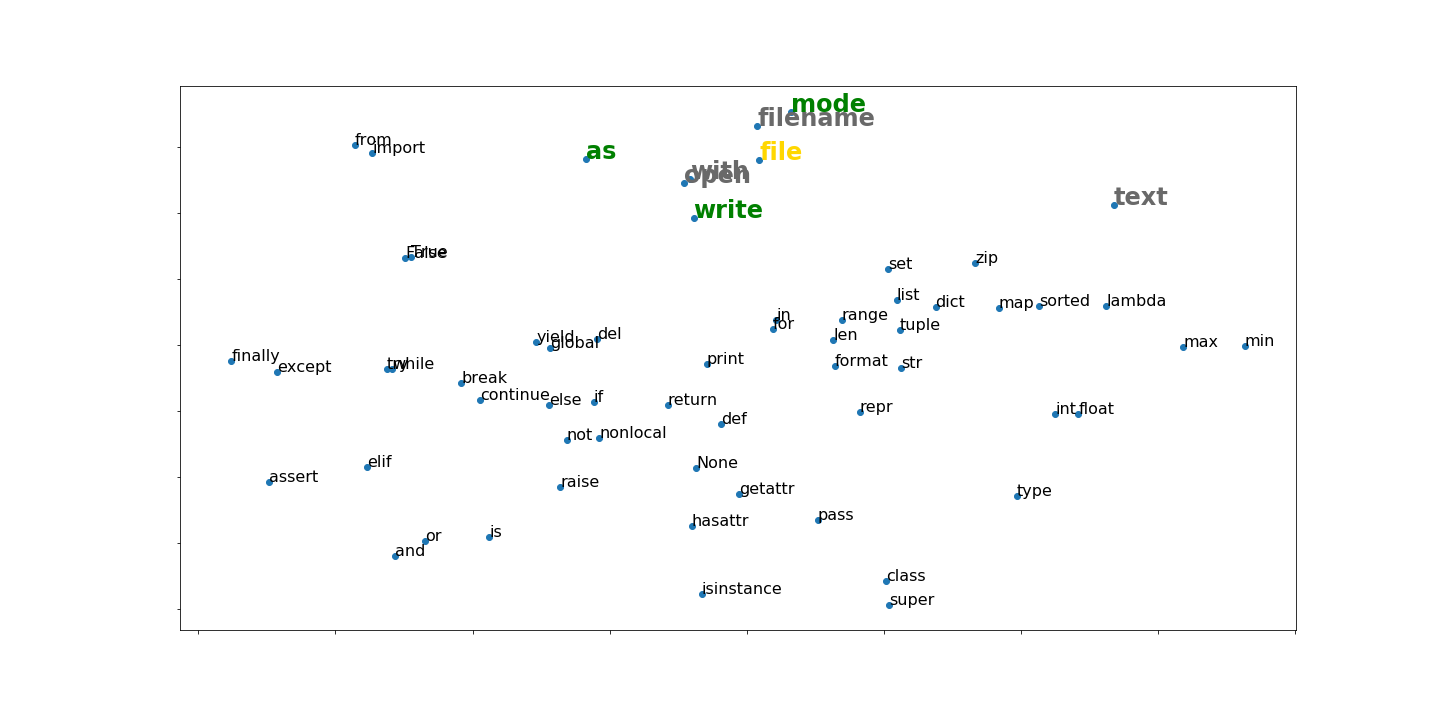
\includegraphics[width=1\textwidth]{figuras/cap-trabalhos-relacionados/code-tsne-output.png}
\caption{Representação em 2D do vetor de representação distribuída de trechos de código-fonte. Imagem gerada através da ferramenta t-SNE. E o vetor de representação distribuída foi criado a partir da amostra de trechos de código-fonte em Python disponibilizada por \cite{yao-2018}. Vetor criado utilizando o \textit{word2vec} com o algoritmo \textit{skip-gram} e o parâmetro \textit{window} com o valor $5$.}
\label{fig:tsne-code-snippet-python}
\end{figure}